\section{Introduction}
\label{sec:intro}

\subsection{A Great Theorem}
The Gauss-Bonnet theorem states that, given a surface, the sum of the curvature
at each point is equal to $2\pi$ times the Euler characteristic.
The theorem is a bridge between many ideas that may
seem separate at first, see \figref{bridge}. 
This bridge allows bidirectional traffic directions.



\begin{figure}[htb]
\centering
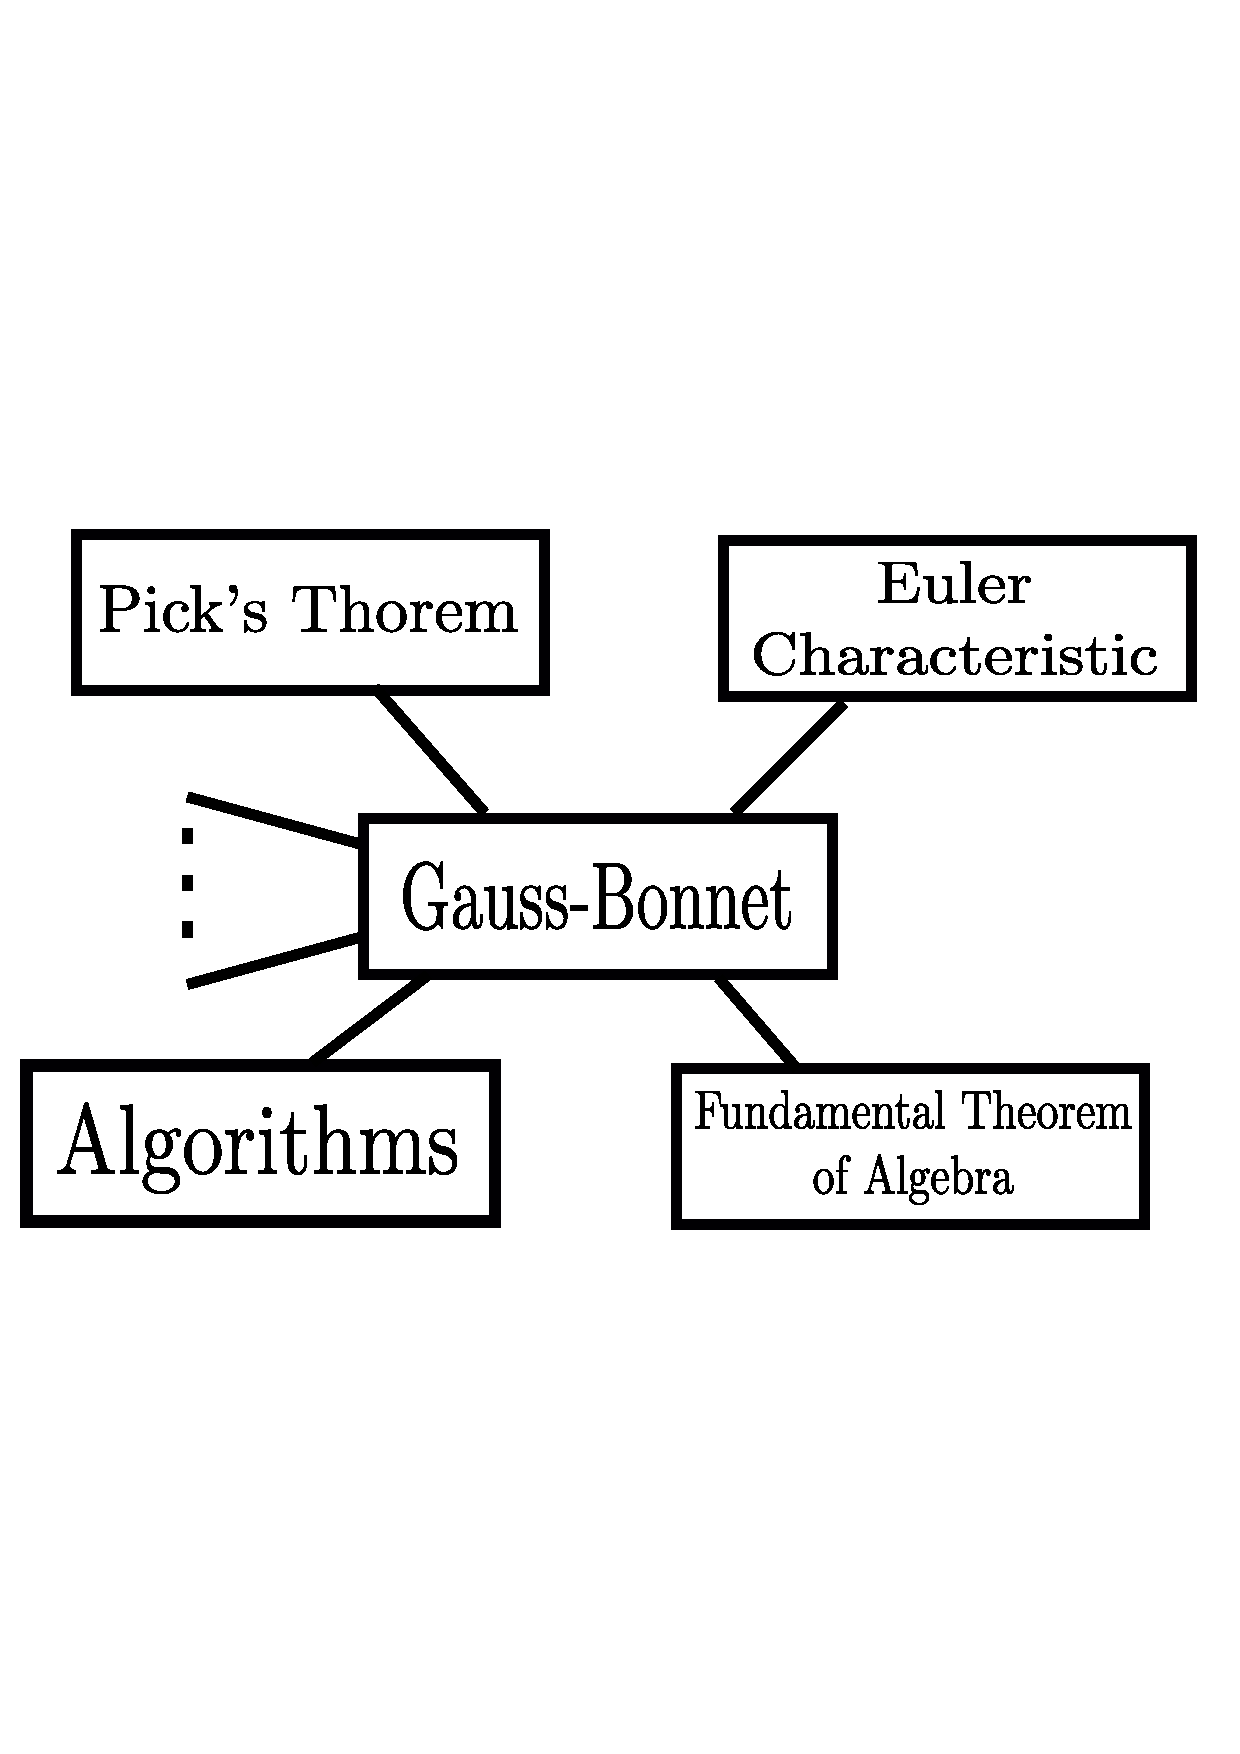
\includegraphics[width=.3\textwidth]{curvature/bridge}
\caption{The Gauss-Bonnet theorem is a star.}
\label{fig:bridge}
\end{figure}

In the book \emph{Using the Borsuk-Ulam Theorem}
\cite{jm08},
Matou\v{s}ek states that a theorem is a great theorem if there are
\begin{enumerate}[(1)]
\item several different equivalent versions,
\item many different proofs,
\item a host of extensions and generalizations, and
\item numerous interesting applications.
\end{enumerate}

By this criteria, the Gauss-Bonnet theorem is a great theorem.
For (1), six\todo{verify} different versions of the theorem are discussed
in \cite{wu_historical_2008}. 
We highlight a version for smooth surfaces in $\RR^3$ and
 several discrete versions for triangulated surfaces. 
 Versions exist for surface with boundary even with cusps on
 the boundary.
 Local and global versions are given in \cite{doc76}.
Versions exist for higher dimensions \cite{guillemin_differential_2010}.
The versions we discuss are extrinsic, meaning they depend on an embedding
into $\R^n$, an intrinsic version, not depending on an embedding,
 is given in \cite{chern_simple_1944}.
 
 
As for (2), the most common proof is to first prove the theorem for simply connected domains
with boundary, then triangulate a surface and add up the contribution from each triangle.
The disadvantage of these proofs is that they do not provide geometric intuition \cite{wu_historical_2008}.
In order to limit the number of definition included in the background,
we give proof using this strategy.
Several fundamentally different proofs exist.
For example, in \cite{guillemin_differential_2010}, 
the Poincar\'{e}-Hopf Theorem is used,
in \cite{doc76,pressley_elementary_2010} Green's theorem is used,
in \cite{levi-bicycle} a theorem based on dual cones is given
and in \cite{grinfeld_introduction_2013}
a proof based on the calculus of
moving surfaces is given.\todo{other versions?}
For (3), two prominent generalizations include
the Chern-Gauss-Bonnet theorem \cite{chern_simple_1944} and the Atiyah–Singer index 
theorem \cite{atiyah_index_1963}.
This work is dedicated to (4).
Most, but not all, of our applications are related to geometric algorithms. 
We only include one of the seven applications given in \cite{doc76}.
For applications to physics see \cite{tirado-physics-apps,gibbons_applications_2008}.
A historical survey of the theorem is given in \cite{wu_historical_2008}.


\subsection{Simple Polygons}
\label{sec:warm-up}

Some of us may remember the following special case
of the Gauss-Bonnet theorem from middle school geometry.
An \EMPH{exterior angle} is created when we extend one of the sides of a polygon.
See \figref{exterior-angles} for an example.
The exterior angle at a vertex can be positive or negative.
If we traverse a polygon and add up the exterior angles
we get $2\pi$ because we perform one revolution.
This is a special case of the Gauss-Bonnet theorem.
No matter how we bend or stretch our polygon,
if the boundary of the polygon stays closed and simple,
the sum the exterior angles will be $2\pi$.

We can also derive a formula for the sum of the angles
of the interior angles.
The proof provides intuition for other proofs we will encounter.
We have
\begin{theorem}\label{thm:triangle}
In the plane, the sum of the interior angles of a triangle is $\pi$.
\end{theorem}
\begin{proof}
Draw a line parallel to one edge through the opposite vertex.
By alternating interior angles in the plane, the sum of the angles
in the triangle equal a straight line.
See \figref{interior-angles} for an example. 
\end{proof}


 \begin{figure}[htb]
         \centering
        \begin{subfigure}[b]{0.35\textwidth}
         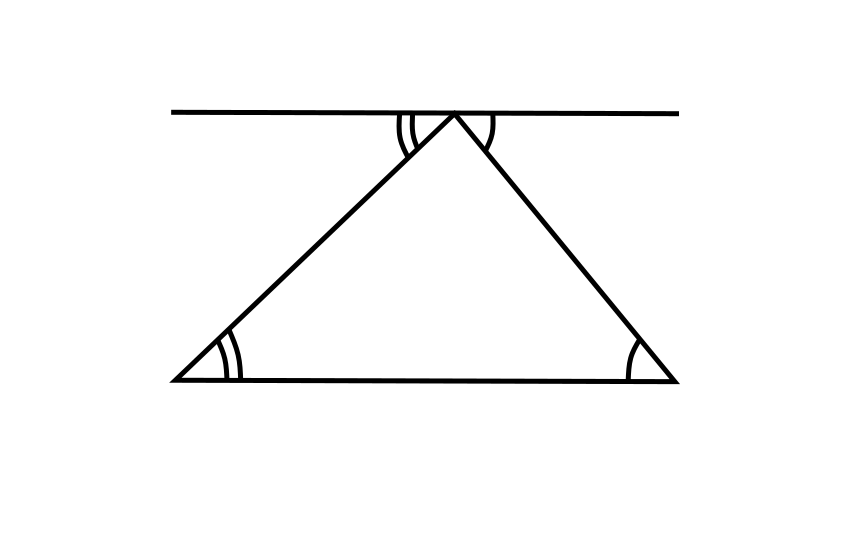
\includegraphics[width=\textwidth]{background/interior-triangle}
         \caption{Interior angles.}
 	 \label{fig:interior-angles}
       \end{subfigure}
         \hspace{1cm}
         \begin{subfigure}[b]{0.25\textwidth}
         \includegraphics[width=\textwidth]{background/exterior-angles-polygon}
         \caption{Exterior angles.}
          \label{fig:exterior-angles}
         \end{subfigure}
		\caption{(a) In the plane, the sum of the interior angles of a triangle is $\pi$
 		and (b) the sum of the exterior angles of a simple
		polygon is $2\pi$. Here
		$\alpha_1+\alpha_2+\alpha_3+\alpha_4+\alpha_5=2\pi$.
 		\label{fig:simple-polygon}}
 \end{figure}

And we have
\begin{corollary}\label{cor:angles}
In the plane, any simple polygon $P$ with $n$ vertices,
the sum of the interior angles of $P$ is $(n-2)\pi$.
\end{corollary}

\begin{proof}
	Consider any simple polygon in the plane $P$ with $n$ vertices. 
	Then $P$ can be triangulated with $n-2$ triangles \cite{orourke_computational_1994}.
	Thus, when we traverse $P$ we go around $n-2$ triangles each contributing
	$\pi$.
\end{proof}

 





On the unit sphere we can determine even more about a polygon 
based on the angles. This is because the sphere is curved.
A triangle on the sphere is shown in \figref{sphere-triangle}.


 \begin{figure}[htb]
         \centering
        \begin{subfigure}[b]{0.35\textwidth}
         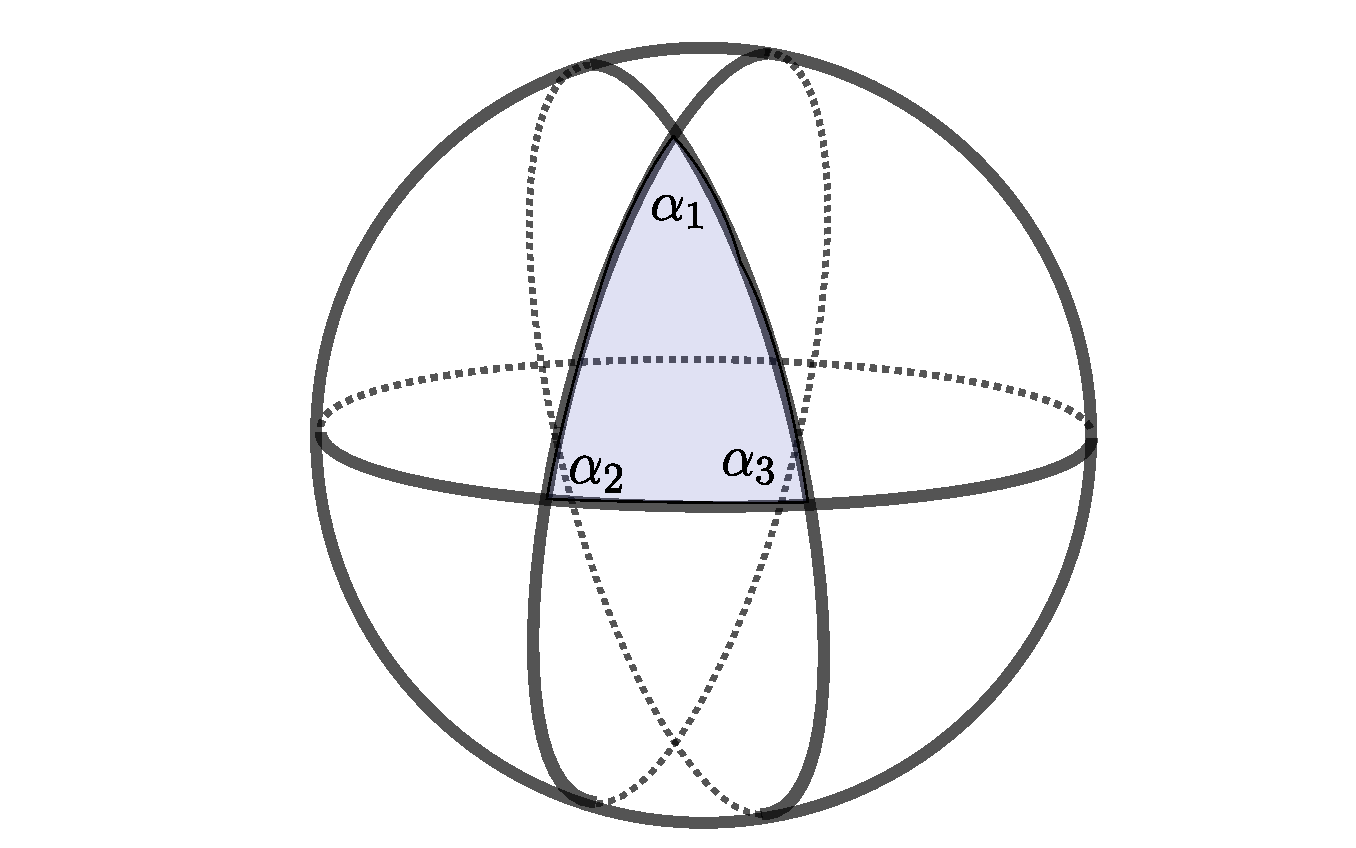
\includegraphics[width=\textwidth]{background/sphere-triangle}
         \caption{Spherical triangle.}
 	 \label{fig:sphere-triangle}
       \end{subfigure}
         \hspace{1cm}
         \begin{subfigure}[b]{0.35\textwidth}
         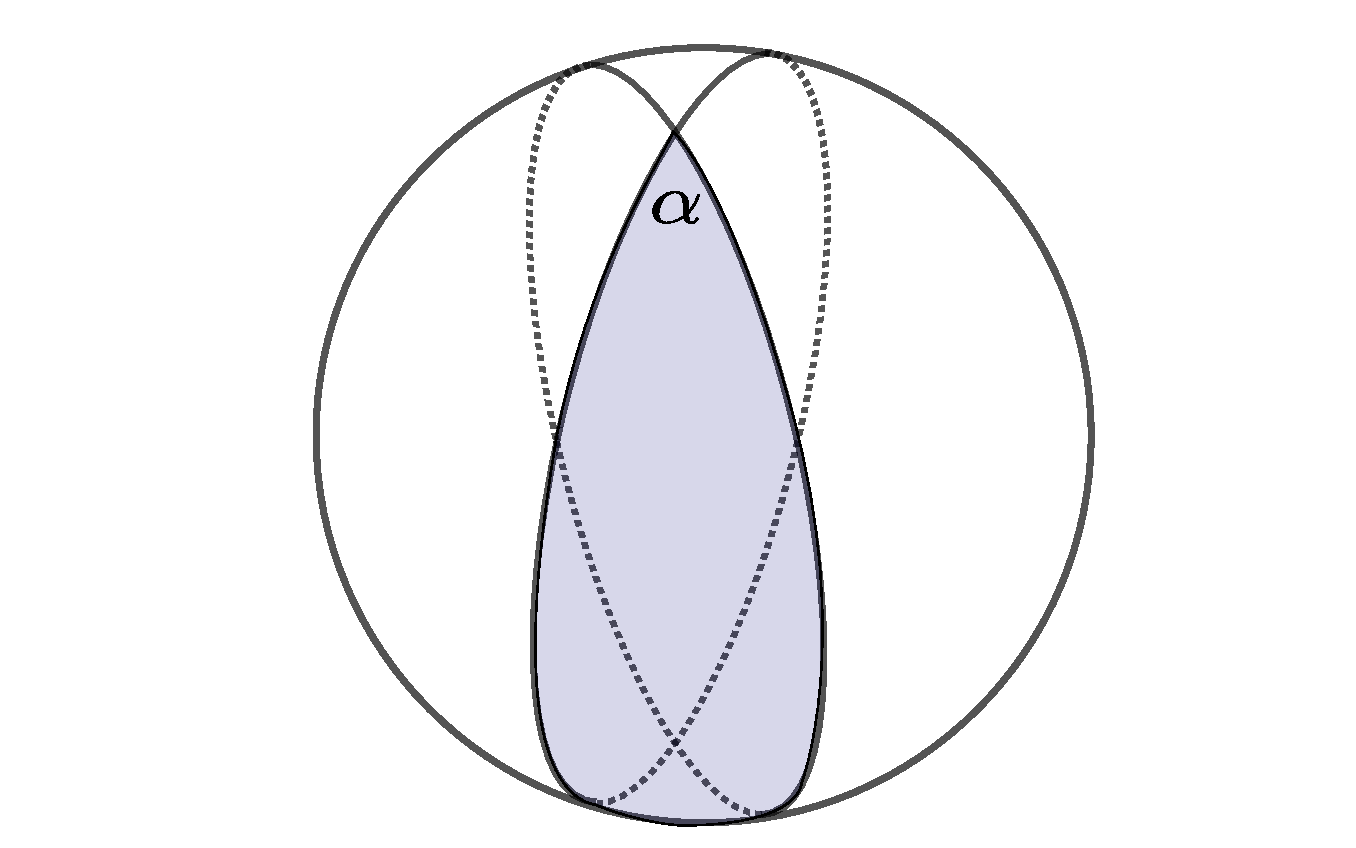
\includegraphics[width=\textwidth]{background/lune}
         \caption{A lune.}
          \label{fig:lune}
         \end{subfigure}
		\caption{(a) A triangle on the sphere.
 		(b) A lune with angle $\alpha$.
 		\label{fig:sphere-lune}}
 \end{figure}
A spherical \EMPH{lune} is the region on a sphere bounded by two half great circles
with angle $\alpha$ the area of a lune is denoted $A(\alpha)$,
 see \figref{lune}.
On the unit sphere, the area of a lune is proportional to $\alpha$. 
If $\alpha=0$ the area is zero and if $\alpha=\pi$ the area is $4\pi$.
We can add the area of two lunes in terms of their angles, 
$A(\alpha_1+\alpha_2)=A(\alpha_1)+A(\alpha_2)$ so $A$ is linear
and  $A(\alpha)=4\alpha.$




The area of a triangle on the sphere is related to the angles.

\begin{lemma}[Area of Spherical Triangle]\label{lem:spherical-triangle}
On the unit sphere, the area of a triangle with interior angles $\alpha_1, \alpha_2, \alpha_3$
is $A=\alpha_1+\alpha_2+\alpha_3-\pi$.
\end{lemma}

\begin{proof}
Any two edges of the the triangle form a lune. The collection of 
all three lunes covers the entire sphere with triangle and the antipodal triangle
are covered three times. The surface area of the unit sphere is $4\pi$.

Thus, $4\pi=2(2\alpha_1+2\alpha_2+2\alpha_3)-6A+2A$
and $A=\alpha_1+\alpha_2+\alpha_3-\pi$.
\end{proof}

As in the plane, any polygon on the sphere with $n$ vertices can be decomposed
into $n-2$ triangles. This gives a formula for the area of a simple polygon
on the sphere with interior angles $\beta_1,\beta_2,\ldots, \beta_n$.

\begin{equation} \label{eqn:sphere-area}
A=(2-n)\pi +\sum_{i=1}^n \beta_i.
\end{equation}







The remainder of this document is organized as follows:
in \secref{background} we introduce definitions and notation. 
We then state two versions of the theorem and prove one of them.
In each subsection of \secref{applications}, we present an application of the theorem.
These subsections are independent.
I hope that the number of applications continues to grow,
please share any that you feel
ought to be included\footnote{\text{bradleymccoy@montana.edu}}.

